In order to obtain optimal performance from the neural networks
given a set of atomistic configurations we need a careful choice of parameters
and neural network architecture. The parameters can be classified as either
training parameters - such as learning rate and force loss coefficient -
or architectural parameters - such as the number of neurons and hidden layers,
or the choice of interaction cutoff radius. The former are important
in the training of the neural network, i.e. adjusting weights and biases
while the latter influence both the training process and the final
deployment of the neural networks on unfamiliar data.
In this section we will be employing a grid search over a set of
parameters, training multiple neural networks on the same data set
and subsequently testing energy and force Root Mean Squared Errors on
a smaller test data set. Generally we will only be training the neural networks
on the energies, since training with forces is much more CPU- and memory-
intensive. However, training with forces would likely affect the final
result and improve the force RMSEs, as we will observe in the following section.
The parameters are unless otherwise specified the defaults listed
in table \ref{table:defaults}.
In their paper on Random Search, \parencite[Bergstra and Bengio]{
    bergstra2012random}
demonstrate that Random Search outperforms Grid Search for dimensions
of search space larger than 3 or 4. However, since we have tested
a small number of parameters (since training and testing is costly)
and we have a general idea of what parameters are appropriate, we
have chosen to employ Grid Search.
AMP has a built in simulated annealing module, which performs
simulated annealing on the weights and biases of the network,
in order to find values for which the loss is lowest.
The annealing is run for every trained neural network
for 2000 steps at the beginning of the training procedure,
with temperatures starting $T_{max} = 20$ and ending $T_{min} = 1$.
Simulated annealing is a suitable algorithm for finding minima
in a complicated energy landscape, and it reduces somewhat
the randomness of initialization so that the results are comparable
without having to perform many runs.

\begin{table}[h]
\begin{tabular}{@{}lll@{}}
\toprule
\multicolumn{3}{l}{Hyperparameters}                                    \\ \midrule
Architecture & Symmetry functions & 12 radial, 20 angular               \\
             & Hidden layers      & (10, 10)                           \\
             & Activation         & Hyperbolic tangent                 \\
             & Cutoff function    & Polynomial, $R_c = 6.0, \gamma = 5.0$
             \\
Training     & Epochs             & 2000                               \\
             & Energy coefficient & 1.0                                \\
             & Force coefficient  & None                                \\
             & Optimizer          & BFGS                               \\ \bottomrule
\end{tabular}
\caption{Training defaults}
\label{table:defaults}
\end{table}

The AMP package provides a set of defaults for most elements,
and these symmetry functions are plotted in figure \ref{fig:default}.
However, we did not feel that these covered the radial and angular space
sufficiently so we constructed our own instead which is what we will
use for training. AMP only provides centered radial functions,
while we use a mix of centered and shifted radial functions
since these have demonstrated higher performance, as is discussed
in the section on symmetry functions.
For the symmetry functions we have chosen a set of 8 uncentered radial,
8 centered radial and 20 angular (G4)
symmetry functions. 
The uncentered radial functions have $\eta$s spaced evenly
from 1 to 20 and are centered at 0. The centered radial functions
are centered evenly from 0.5 to $R_c - 0.5$ with $\eta = 5.0$.
The angular functions have $\eta$s spaced evenly from
0.01 to 3 with $\zeta = 1$ and $\gamma = \pm 1$.
These symmetry functions are displayed in figure \ref{fig:selected}.
We also choose to employ the polynomial cutoff introduced in AMP,
since this has a wider range of values inside the cutoff boundary.

\begin{figure}[!tbp]
\begin{adjustbox}{max width=1.2\linewidth,center}
\centering
  \begin{subfigure}[b]{0.55\textwidth}
      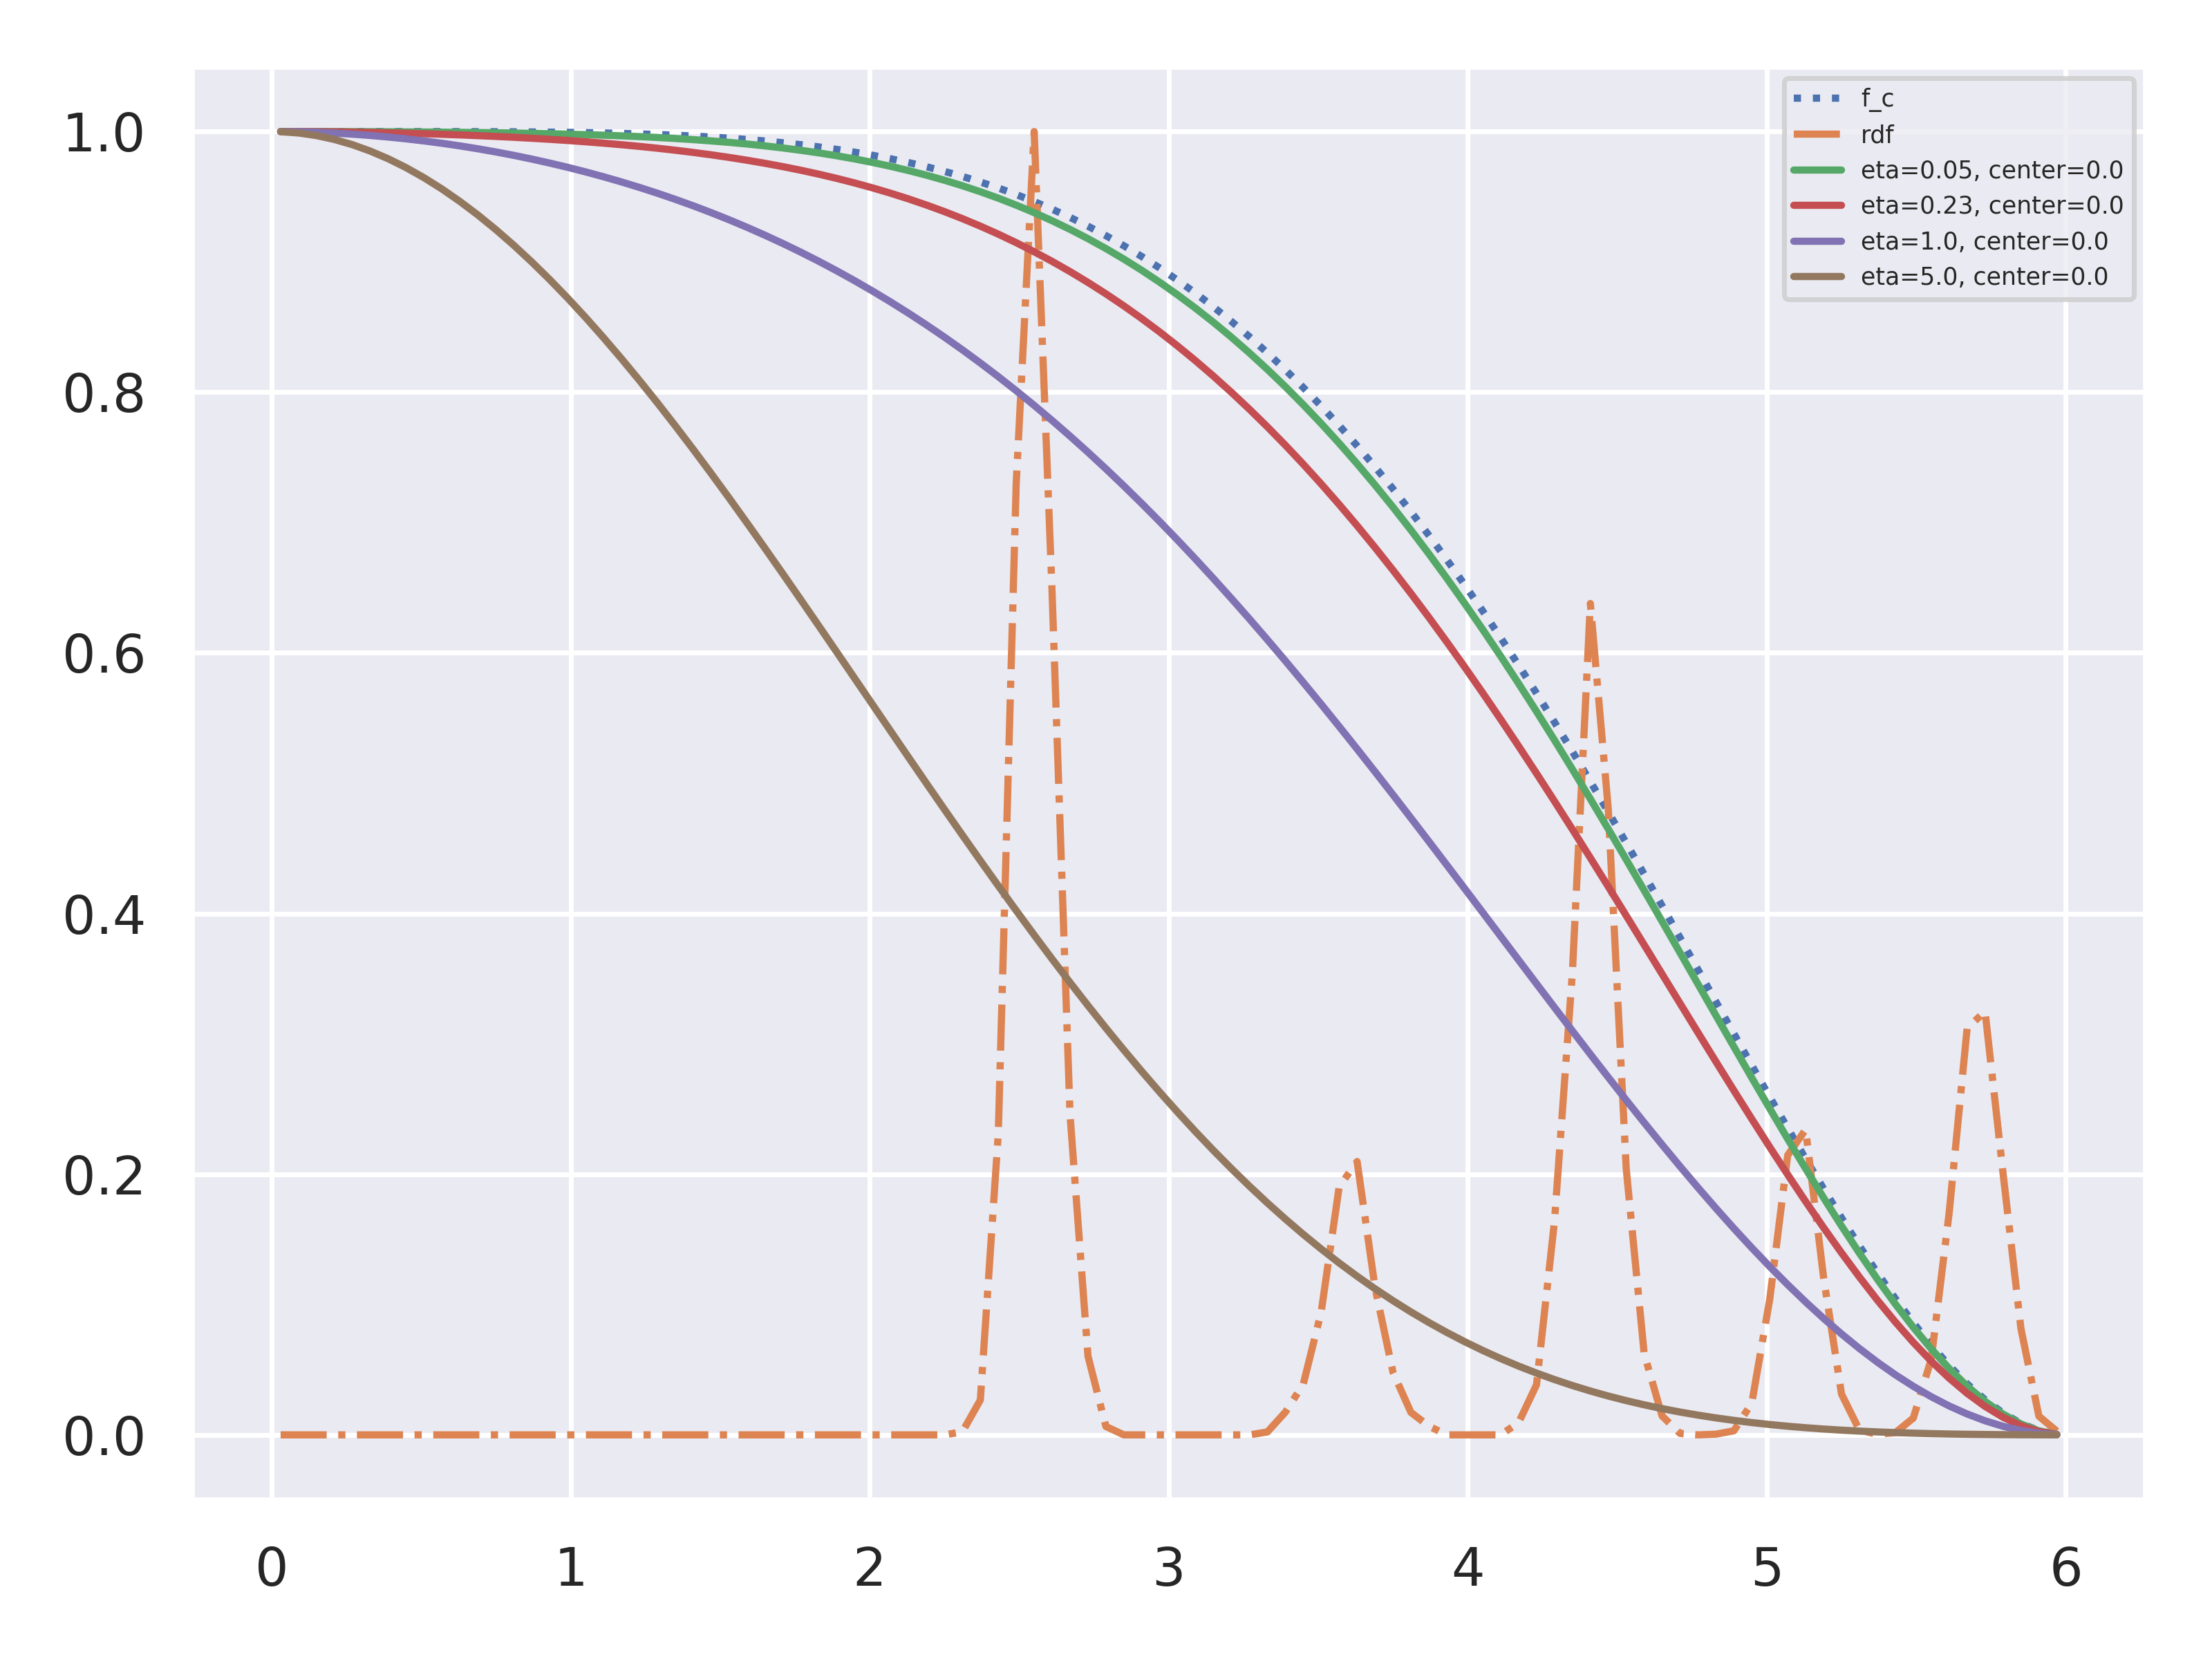
\includegraphics[width=\textwidth]{Default-rad.png}
    \caption{Flower one.}
    \label{fig:f1}
  \end{subfigure}
  \hfill
  \begin{subfigure}[b]{0.55\textwidth}
      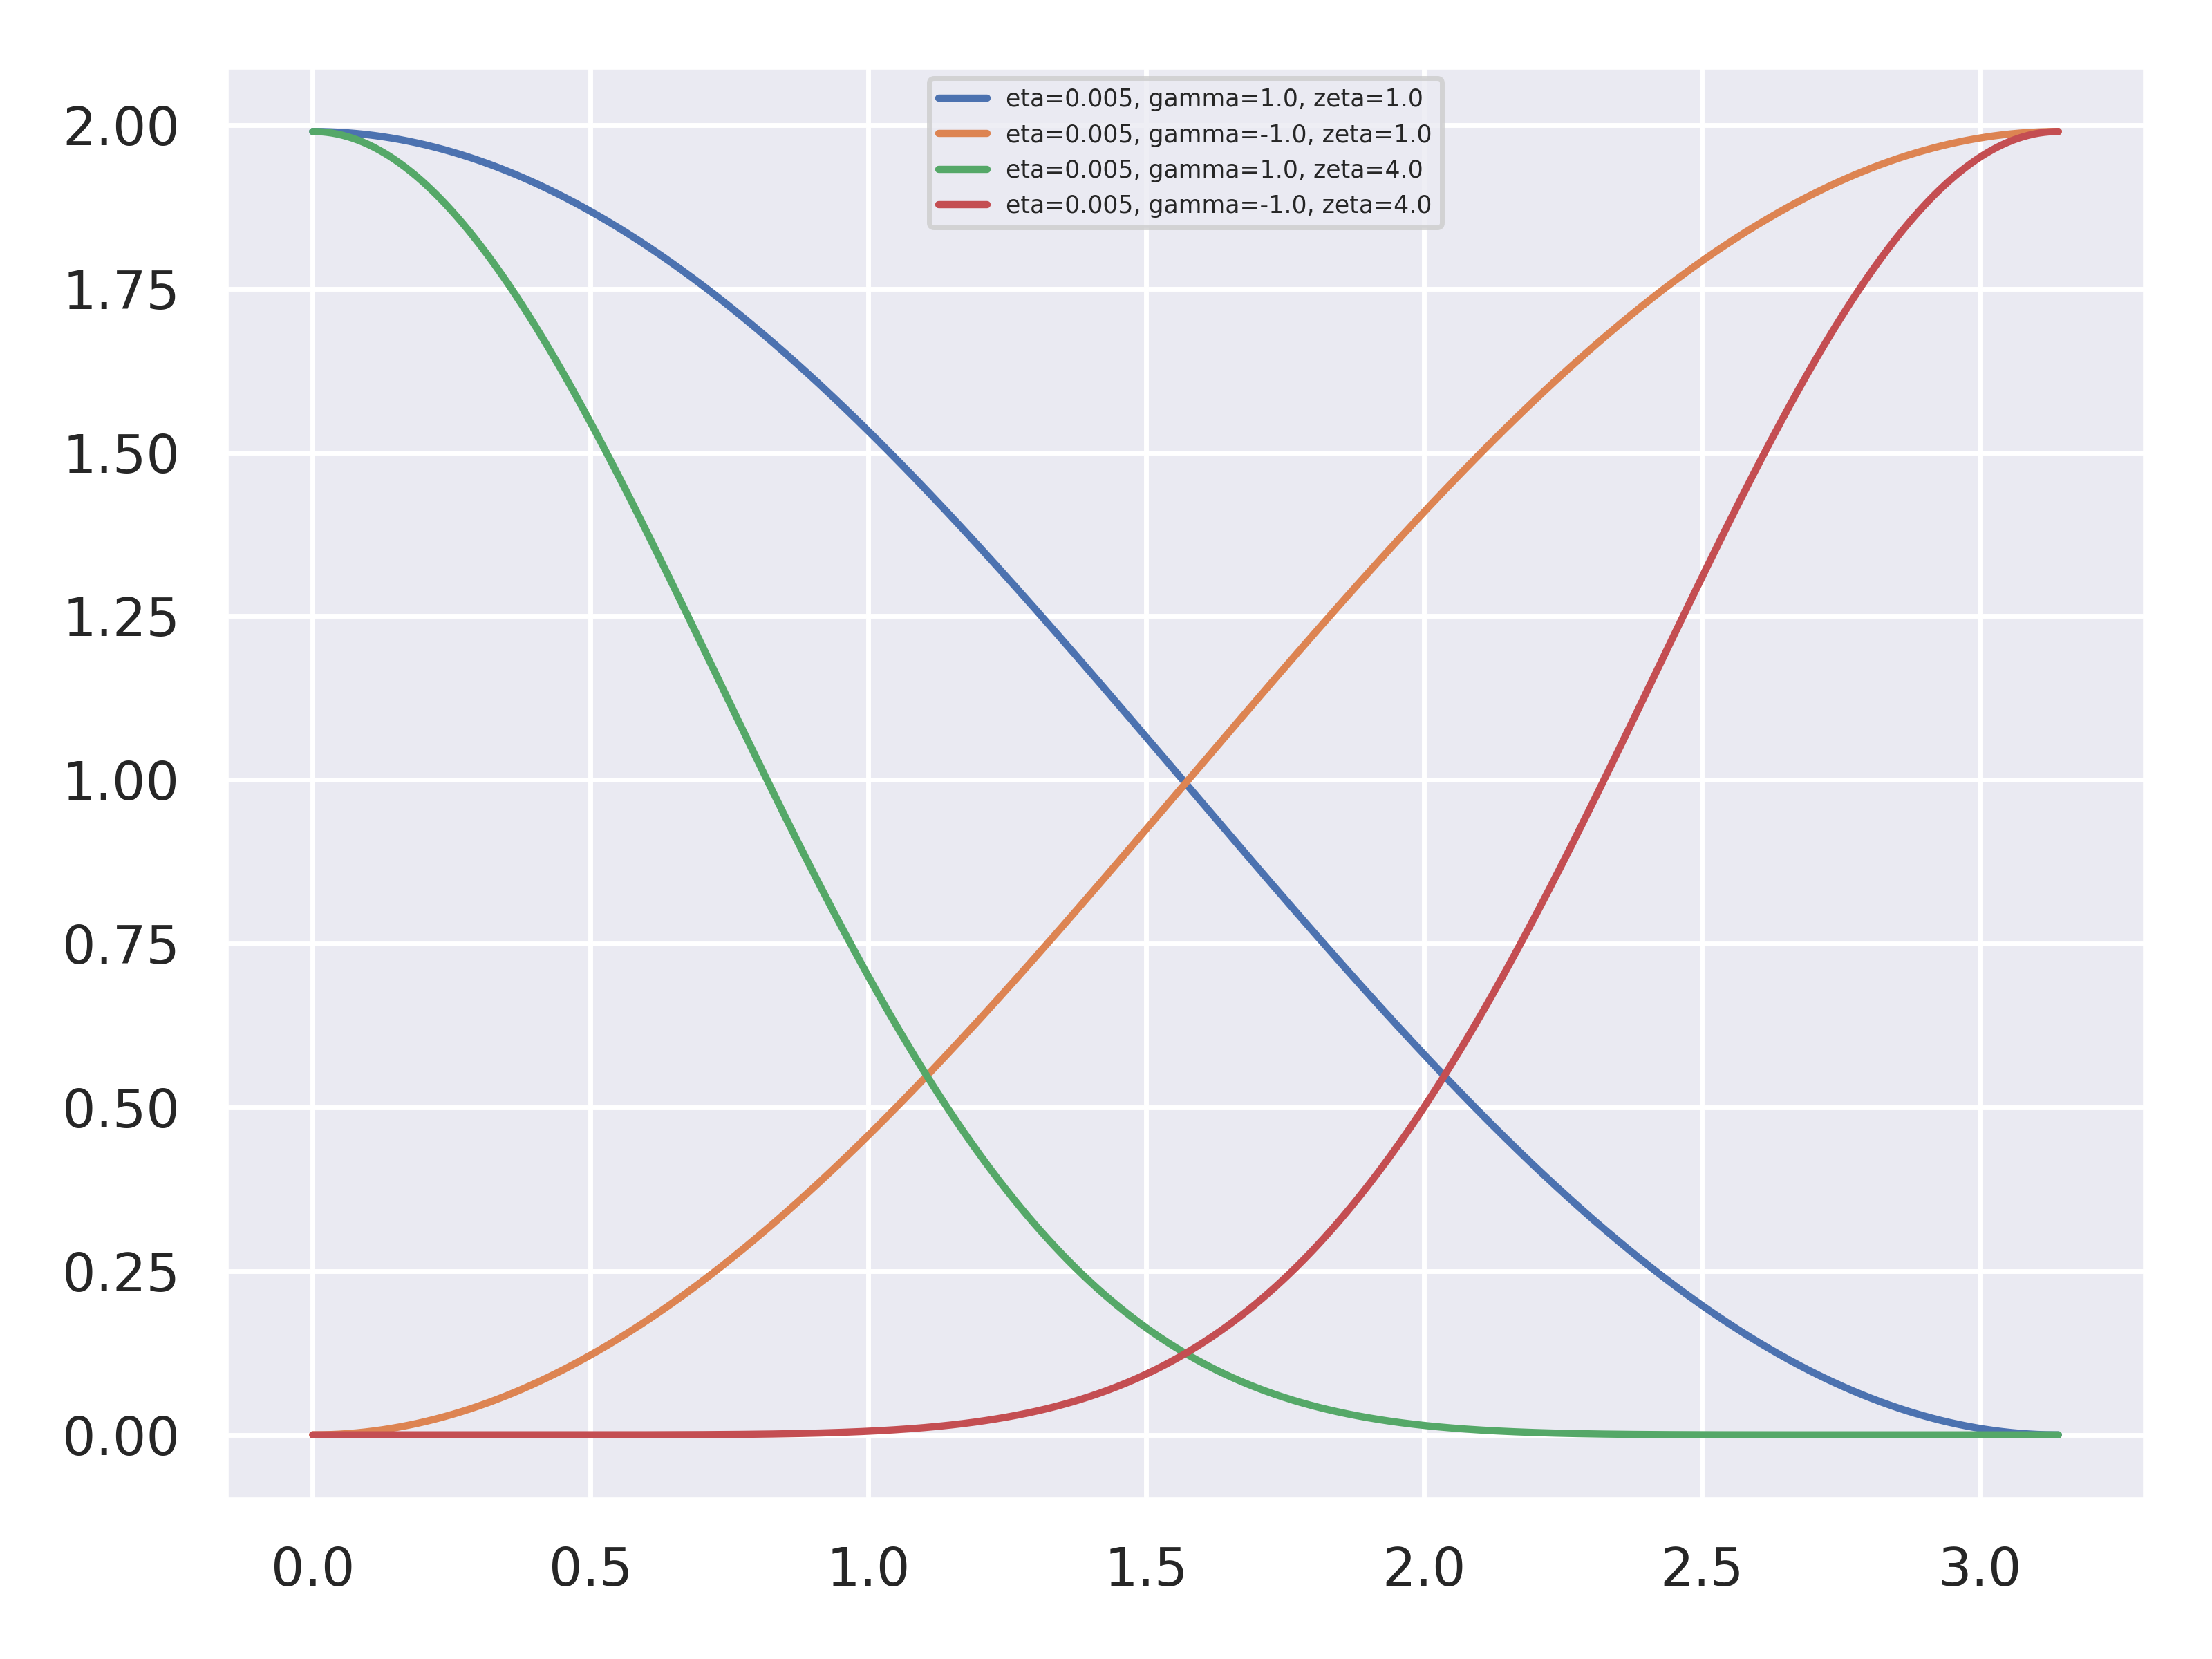
\includegraphics[width=\textwidth]{Default-ang.png}
    \caption{Flower two.}
    \label{fig:f2}
  \end{subfigure}
\end{adjustbox}
\caption{My flowers.}
    \label{fig:default}
\end{figure}

\begin{figure}[!tbp]
\begin{adjustbox}{max width=1.2\linewidth,center}
\centering
  \begin{subfigure}[b]{0.55\textwidth}
      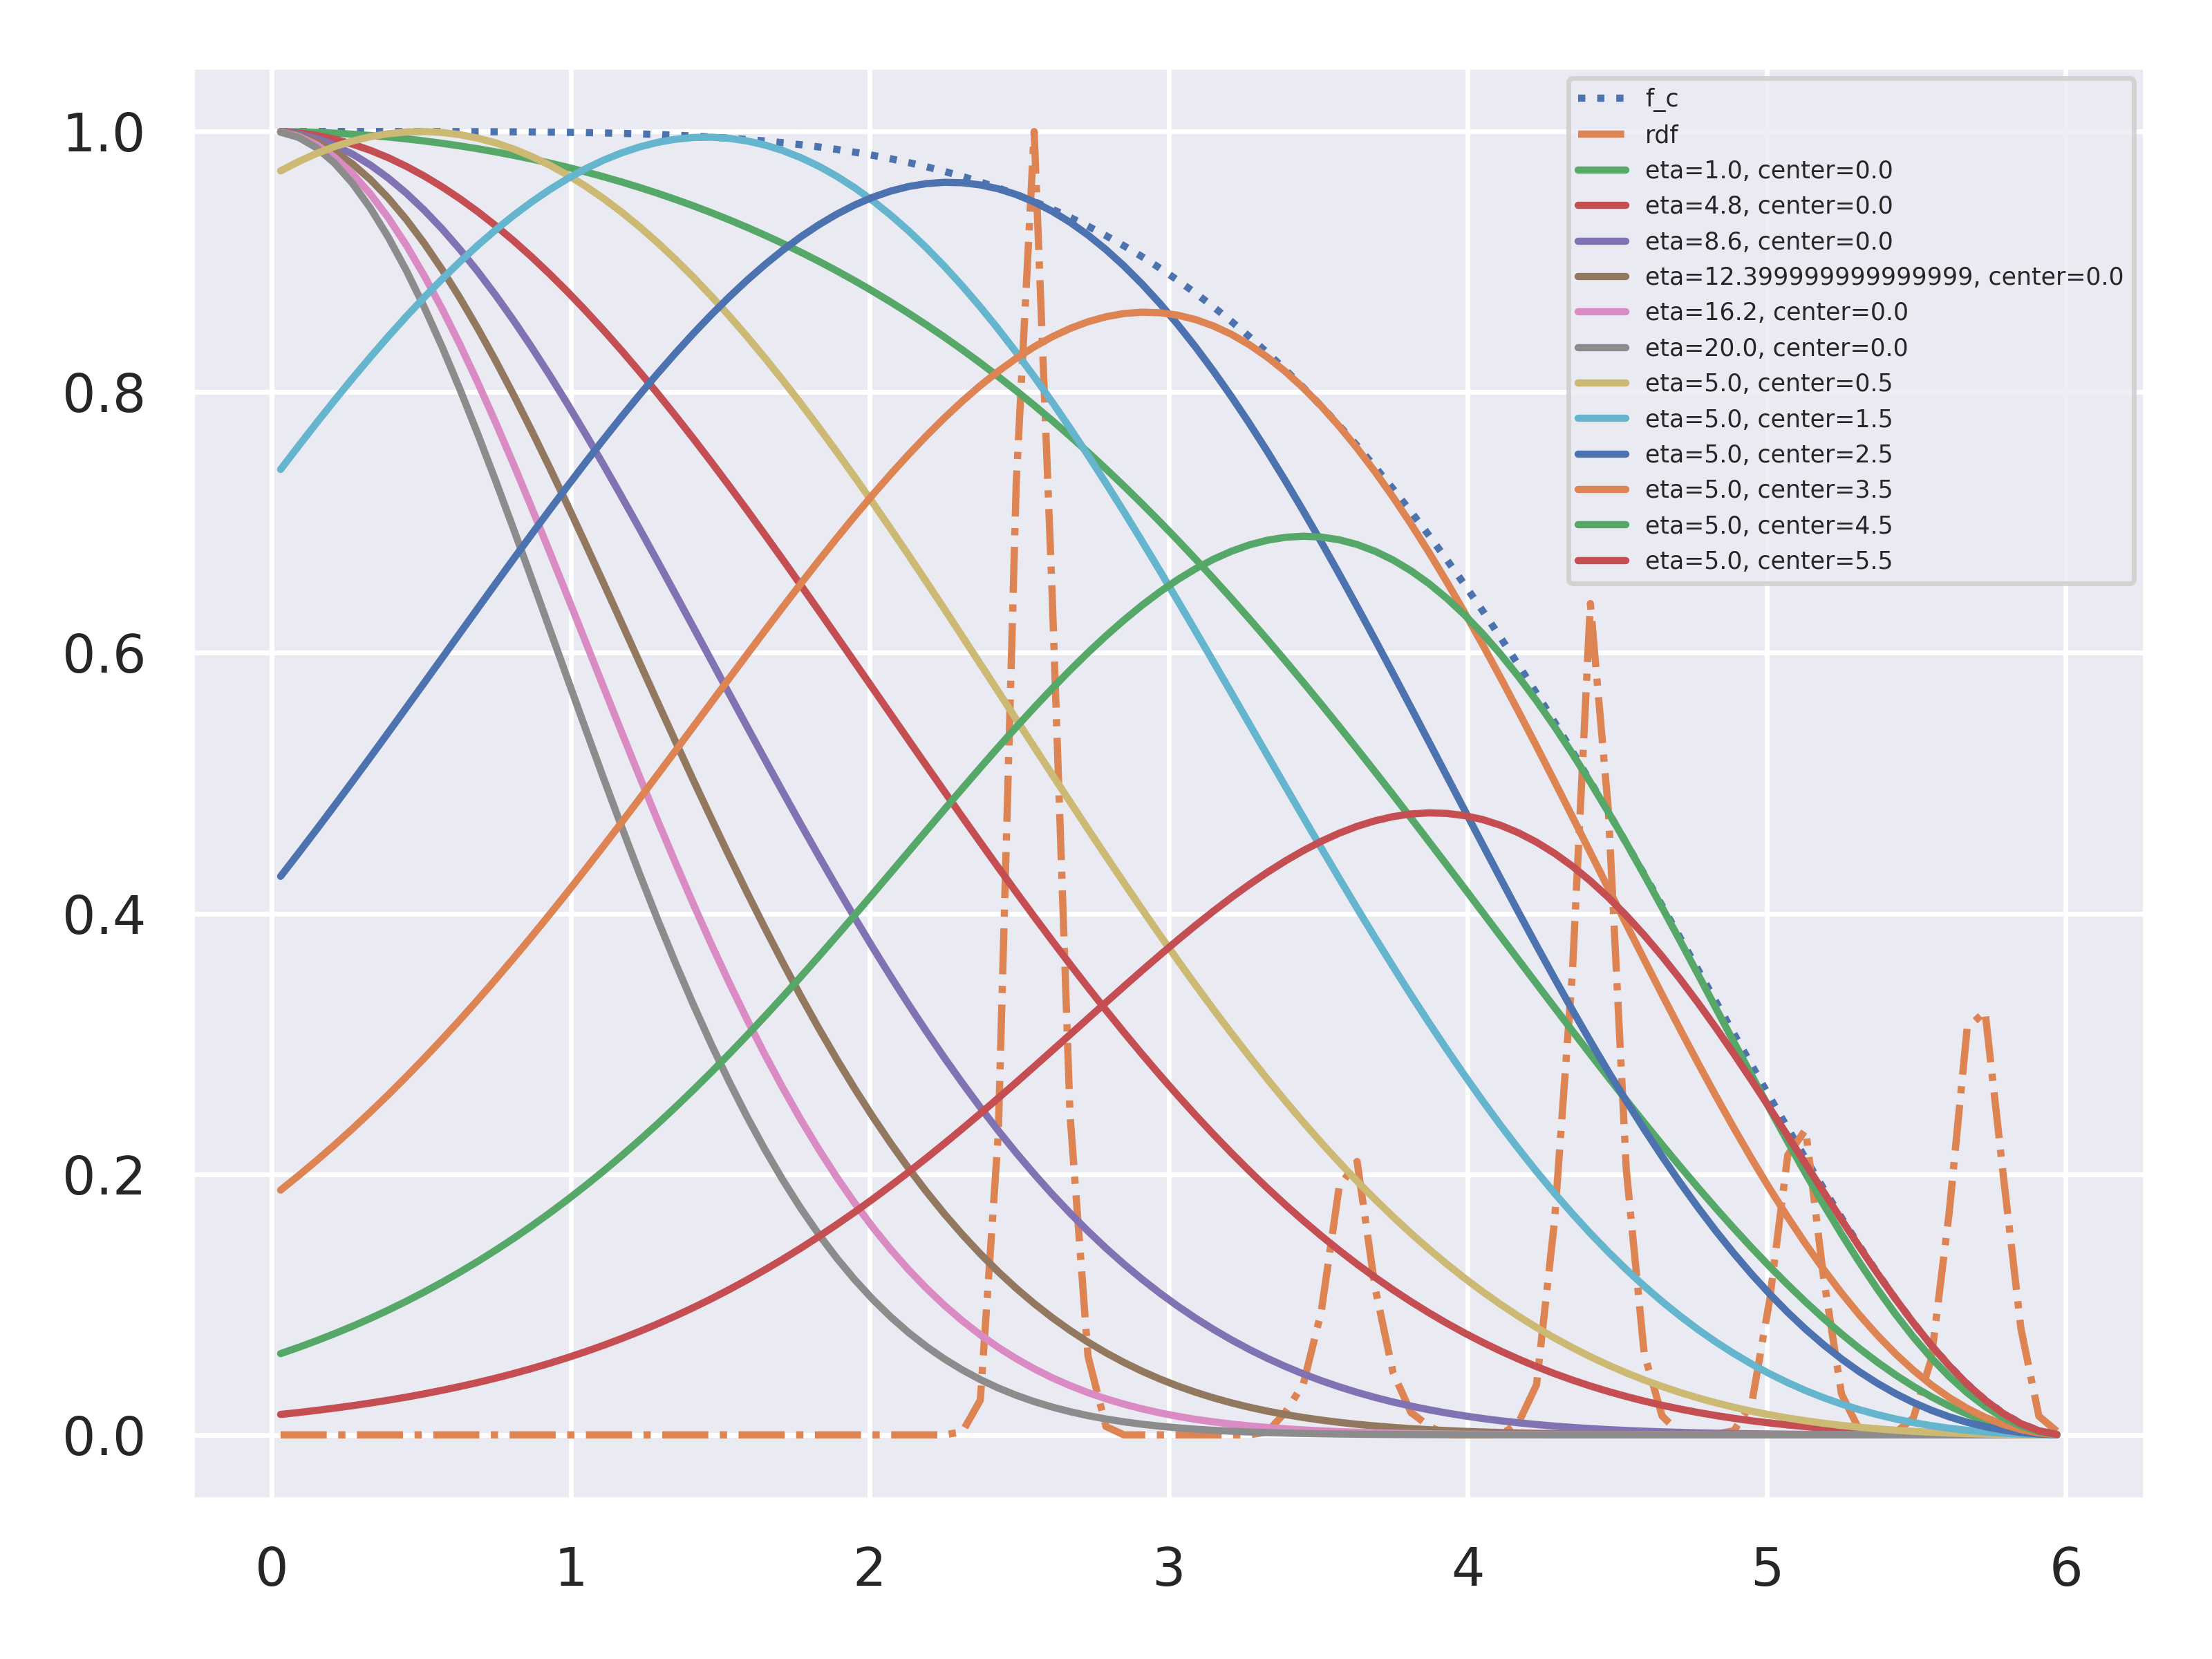
\includegraphics[width=\textwidth]{Selected-rad.png}
    \caption{Flower one.}
    \label{fig:f1}
  \end{subfigure}
  \hfill
  \begin{subfigure}[b]{0.55\textwidth}
      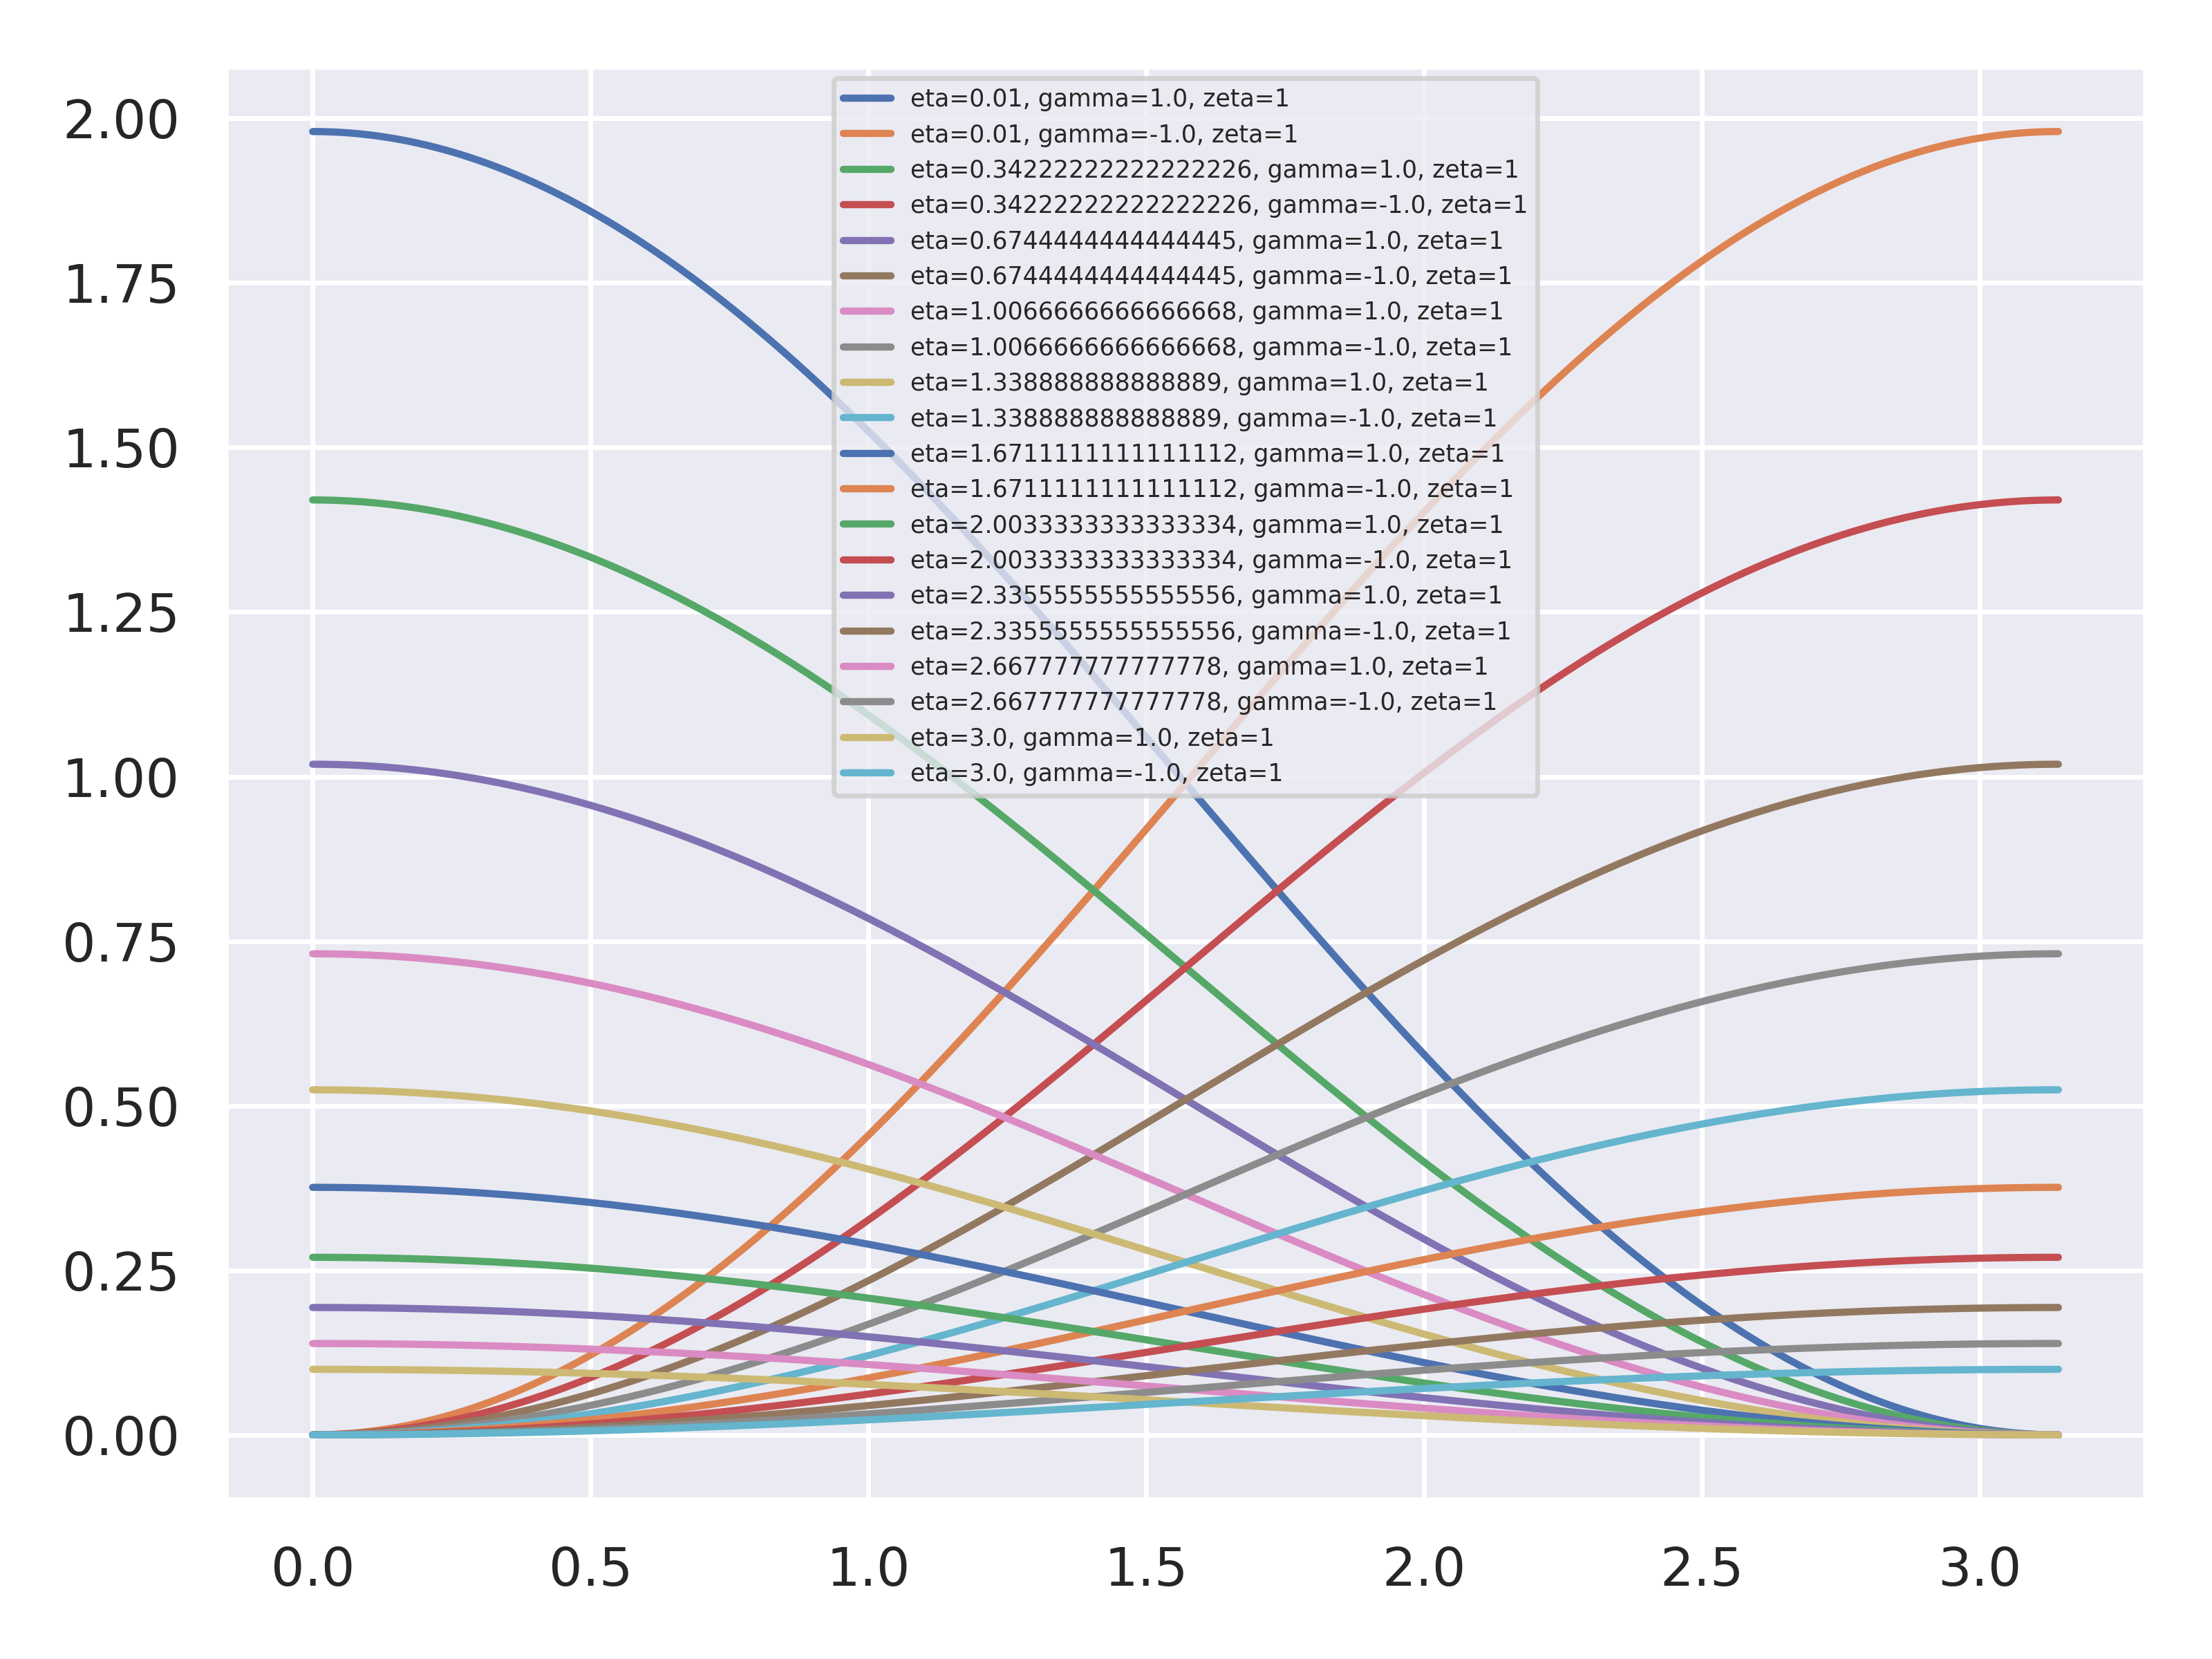
\includegraphics[width=\textwidth]{Selected-ang.png}
    \caption{Flower two.}
    \label{fig:f2}
  \end{subfigure}
\end{adjustbox}
\caption{My flowers.}
    \label{fig:selected}
\end{figure}

\subsection{Force training}
When training the neural networks we have the choice of whether
to incorporate the forces into our loss function, or only fit
the neural network to the potential energy. By default, unless
we have access to a per-atom energy every configuration is labeled
with only a single number for a potentially large number of atoms,
which limits the improvement in loss metrics for every epoch
and the final result. If instead we incorporate the forces into the
loss we have potentially $3N + 1$ labels for every epoch,
which provides a lot more information for weight updates.
In the previous chapter we also showed how adding derivatives to
the loss function could significantly improve the accuracy of the
derivatives. Since the forces determine the trajectories generated
from molecular dynamics we would expect we would expect much better
accuracy and numerical stability if we could improve the fit of
the derivatives.
The real drawback is the calculation of the derivatives in the input layer,
aka the fingerprintprimes, of which there are a lot for every coordinate
and input symmetry function, and they consume a lot of disk space and memory.
\par
In order to test the performance of neural networks
we trained with and without forces on a set of test images.
A system of copper atoms is generated in the face-centered cubic (FCC)
configuration with 4 atoms in the unit cell and $3 \times 3 \times 3$
unit cells for a total of $4 \cdot 3^3 = 108$ atoms. The
atoms are given velocities from the Maxwell-Boltzmann distribution
corresponding to a temperature of 500 Kelvin. The potential we will
be using is the Effective Medium Theory (EMT), which has a very
fast Fortran implementation in the ASE software package\footnote{
\url{https://wiki.fysik.dtu.dk/asap/asap}}.
The training trajectory is ran for $5 \cdot 10^4$ steps with
a timestep of $\Delta t = 1$fs and written to file every 100 steps
for a total of 500 atomic configurations. The test trajectory is
integrated for $1 \cdot 10^4$ steps for a total of 100 atomic configurations.

\begin{figure}[!tbp]
\begin{adjustbox}{max width=1.2\linewidth,center}
\centering
  \begin{subfigure}[b]{0.55\textwidth}
      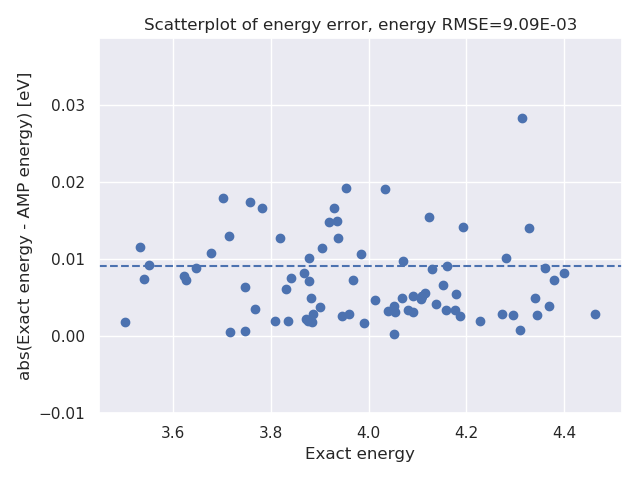
\includegraphics[width=\textwidth]{energy_noforcetrain.png}
    \caption{Flower one.}
    \label{fig:f1}
  \end{subfigure}
  \hfill
  \begin{subfigure}[b]{0.55\textwidth}
      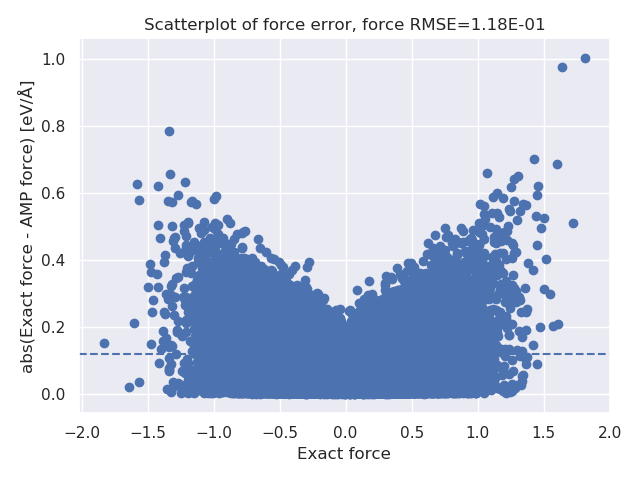
\includegraphics[width=\textwidth]{force_noforcetrain.png}
    \caption{Flower two.}
    \label{fig:f2}
  \end{subfigure}
\end{adjustbox}
\caption{My flowers.}
    \label{fig:noforcetrain}
\end{figure}

\begin{figure}[!tbp]
\begin{adjustbox}{max width=1.2\linewidth,center}
\centering
  \begin{subfigure}[b]{0.55\textwidth}
      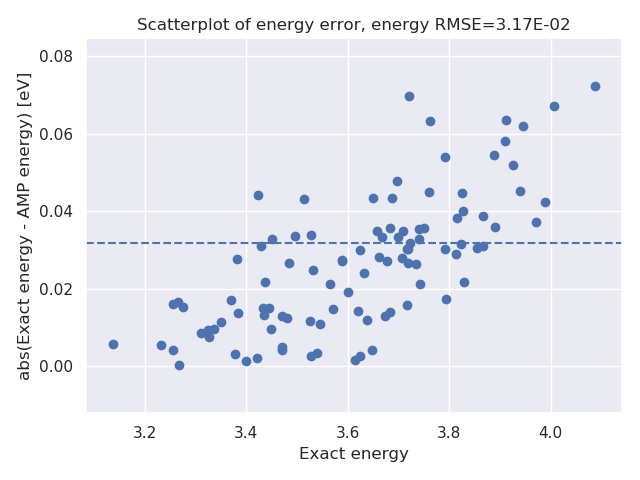
\includegraphics[width=\textwidth]{energy_forcetrain.png}
    \caption{Flower one.}
    \label{fig:f1}
  \end{subfigure}
  \hfill
  \begin{subfigure}[b]{0.55\textwidth}
      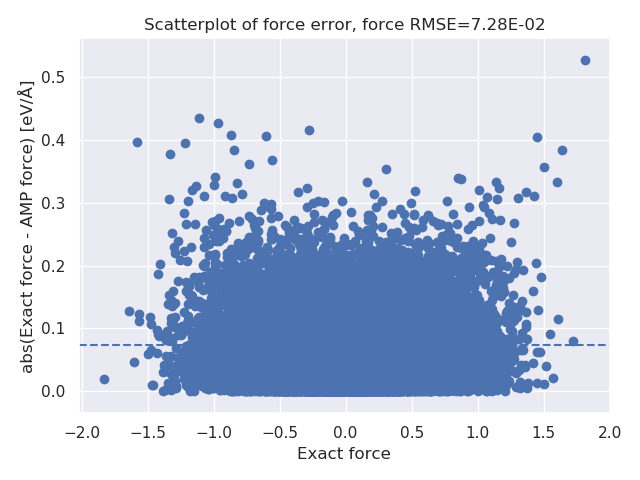
\includegraphics[width=\textwidth]{force_forcetrain.png}
    \caption{Flower two.}
    \label{fig:f2}
  \end{subfigure}
\end{adjustbox}
\caption{My flowers.}
    \label{fig:forcetrain}
\end{figure}

In figure \ref{fig:noforcetrain} we have created a scatterplot
of the energies and forces vs the absolute error, and labeled
the plots with the energy and force RMSEes.
We observe that the potential energies can achieve fairly
low error values of approximately 0.02 to 0.10 eV, and the
result does not depend very much on the value of the exact potential
energy.
The force error however is approximately three orders of magnitude
larger, which echoes some of the concerns raised in the previous
chapter with fitting derivatives. The forces produced by the neural
network are still not dependent on the exact value of the force.
\par
In figure \ref{fig:forcetrain} we have a scatterplot of energies
and forces generated from a force-trained neural network.
While the error in the potential energy is now an order of magnitude higher,
the error in the forces is now two orders of magnitude smaller.
This is arguably a very good tradeoff, since the force error matters
much more for long molecular dynamics trajectories, and will make
any simulation requiring large amounts of data much more stable.
However, force training is as mentioned much costlier in terms
of memory and CPU hours. Instead of training with forces on the full
set of images, we instead suggest training on a large amount of configurations
with only the energies (and arguably a small amount of atoms, since
the ratio of fingerprints to labels is higher), and subsequently training
with forces on a smaller set of images in order to improve the force fit,
at some cost to the energy fit.

\subsection{Activation, hidden layers}
In order to test different network architectures
we test different values of the activation functions, and the number
of hidden layers and nodes. 
At this range of values, we do not expect a large variation in the performance,
while larger neural networks with a large amount of hidden layers
would be expected to overfit the training data and perform
poorly on unseen data.
In the paper Efficient Backprop by \parencite[Lecun et al.]{
lecun2012efficient} the authors suggest that the hyperbolic
tangent outperforms the sigmoid, since the derivatives
are larger, which provides more efficient training.
The hyperbolic tangent is somewhat more computationally costly,
however this is not a big consideration for our neural networks
overall, since they are quite small and can be evaluated
relatively fast.
To test different architecturesj a copper system of $4 \cdot 2^3 = 32$
atoms is generated and integrated for $8 \cdot 10^4$ steps
with a timestep of $\Delta t = 1.0$fs
and written to file every 100 steps for a total of 800 training images.
By the same procedure we also obtain 100 test images.
The velocities are generated
according to a Maxwell-Boltzmann distribution with a temperature
of 500 Kelvin. The results are shown in table \ref{table:act-hidden}.
The network is trained only on energies, while for the test set
we calculate the energy and force Root Mean Squared Errors (RMSEs).

\begin{table}
\begin{tabular}{lrr}
\toprule
Activation/Hidden layers &  Energy RMSE &  Force RMSE \\
\midrule
               tanh-[10] &     3.54E-03 &    5.84E-02 \\
               tanh-[20] &     2.01E-03 &    1.47E-01 \\
               tanh-[30] &     1.46E-03 &    9.91E-01 \\
               tanh-[40] &     1.70E-03 &    9.35E-01 \\
           tanh-[10, 10] &     1.84E-03 &    1.97E-01 \\
           tanh-[20, 10] &     2.91E-03 &    9.66E-02 \\
           tanh-[30, 10] &     3.51E-03 &    8.29E-02 \\
           tanh-[40, 40] &     1.80E-03 &    1.86E-01 \\
            sigmoid-[10] &     1.85E-03 &    9.44E-01 \\
            sigmoid-[20] &     3.73E-03 &    3.25E-01 \\
            sigmoid-[30] &     1.79E-03 &    1.01E+00 \\
            sigmoid-[40] &     2.09E-03 &    2.54E-01 \\
        sigmoid-[10, 10] &     1.93E-03 &    5.98E-01 \\
        sigmoid-[20, 10] &     1.83E-03 &    2.26E-01 \\
        sigmoid-[30, 10] &     1.52E-03 &    1.99E+00 \\
        sigmoid-[40, 40] &     1.94E-03 &    3.36E-01 \\
\bottomrule
\end{tabular}
\caption{Training defaults}
\label{table:act-hidden}
\end{table}

From the results we can see that the results do not
differ significantly. The larger networks may perform somewhat
better on the energy, but this is also somewhat influenced by the stochasticity
of random initialization. For the hyperbolic tangent using
a single hidden layer of 10 nodes we also achieve a fairly
low value on the force RMSE, though the network has not been trained
on forces, but this also matches our intuition that the network
should not be very large, with the hyperbolic tangent outperforming
the sigmoid. For the remainder of this thesis we have settled
on these values for the neural network, though it remains
to be seen if a larger network trained for longer could outperform
the smaller models.

\subsection{Cutoff radius}
The cutoff radius defines the boundary outside of which no interactions
between atoms take place, and the magnitude of the interactions
which take place within. We therefore expect it to have a reasonable
effect on the final result. Ideally we might like all atoms to interact,
as they plausibly do in the real world. However there is a tradeoff
between the accuracy and speed when calculating fingerprints and
fingerprint derivatives, with substantial CPU and memory cost the
larger the cutoff radius, and accuracy can also be impacted if any
atom interacts with an atom which in actuality does not have a substantial
energy and force contribution.
In their original paper on AMP by \parencite[Khorshidi and Peterson]{
khorshidi2016amp}, the authors suggest an alternative cutoff
function to the cosine suggested by Behler and Parrinello
which covers a wider range of values within the cutoff boundary
and can reproduce the cosine at certain values of $\gamma$.

\begin{equation}
    f_c(r) =
    \begin{cases}
        1 + \gamma (r / R_c)^{\gamma + 1} - (\gamma + 1)
        (r / R_c)^{\gamma} & r \leq R_c \\
        0 & r > R_c
    \end{cases}
\end{equation}

We choose a value of $\gamma = 5.0$ since it has a substantially wider
range than the cosine, and compare the two for different cutoff radii.
In figure \ref{fig:copper_rdf} we have plotted the radial distribution
function of the copper atoms governed by the EMT potential.
We see that the system is strongly peaked at distances of approximately
2 and 4 Ångstrøm, with smaller peaks in between and beyond.
It is therefore reasonable to assume that a cutoff between 4
and 8 Ångstrøm would perform well, without sacrificing too much
accuracy.
As in the previous section we produce a system with 32 atoms, with
800 training configurations and 200 test configurations. The network
is only trained on the energy, since this is substantially cheaper,
and then the network is evaluated on the energy and force RMSE
on the test set. The results are presented in \ref{table:cutoffs}.

\begin{table}
\begin{tabular}{lrr}
\toprule
         Cutoff &  Energy RMSE &  Force RMSE \\
\midrule
     Cosine-2.0 &     2.22E-01 &    4.00E-01 \\
 Polynomial-2.0 &     2.22E-01 &    4.00E-01 \\
     Cosine-3.0 &     4.31E-03 &    3.42E-01 \\
 Polynomial-3.0 &     4.22E-03 &    3.54E-01 \\
     Cosine-4.0 &     8.41E-04 &    1.41E-01 \\
 Polynomial-4.0 &     7.92E-04 &    1.74E-01 \\
     Cosine-5.0 &     3.74E-04 &    1.19E-01 \\
 Polynomial-5.0 &     4.94E-04 &    1.40E-01 \\
     Cosine-6.0 &     2.01E-03 &    8.19E-02 \\
 Polynomial-6.0 &     2.48E-03 &    6.93E-02 \\
     Cosine-7.0 &     3.21E-03 &    1.50E-01 \\
 Polynomial-7.0 &     7.16E-03 &    4.66E-02 \\
     Cosine-8.0 &     3.14E-03 &    2.70E-01 \\
 Polynomial-8.0 &     5.95E-03 &    8.90E-01 \\
\bottomrule
\end{tabular}
\caption{Cutoffs}
\label{table:cutoffs}
\end{table}

\begin{figure}
    \centering
    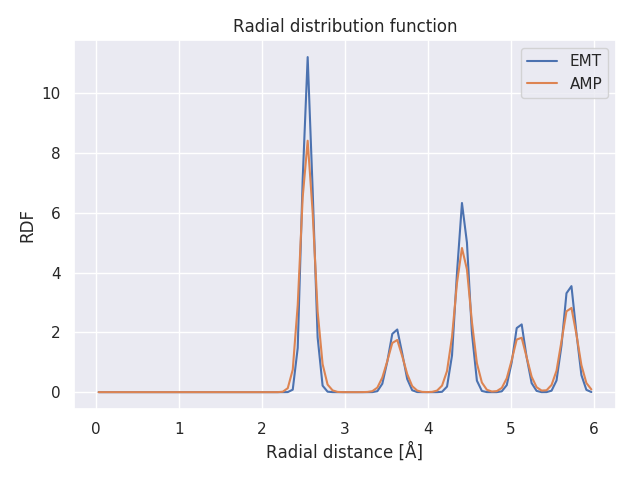
\includegraphics[width=\linewidth]{copper_rdf.png}
    \caption{Copper RDF}
    \label{fig:copper_rdf}
\end{figure}

From the energy RMSEs we can see that the middle values of the
cutoff produce the lowest values. This is likely due to some kind
of overfitting, such that better values are obtained by considering
fewer atoms more strongly. The intermediate values also
seem to produce somewhat lower values of the force RMSE,
of which the lowest is the polynomial with a cutoff of 7 Ångstrøm.
The differences between the cosine and the polynomial do not
appear very large, though the polynomial may obtain marginally
lower values of the force RMSE. We do not that there is a substantial
stochastic element in these tests, and also that longer training
periods may have produced more substantial differences, however
training is costly in terms of CPU time. For the remainder
of this thesis we settled on the polynomial with a cutoff of 6 Ångstrøm,
while the cosine may have performed just as well.
We also note that since the cutoff radius defines a sphere
with a volume $V \propto R_c^3$, the average number of neighbors and therefore
calculations increases substantially with the cutoff radius.

\subsection{Symmetry functions}
The symmetry functions determine the local environment of every atom,
which is then fed through and backpropagated through a neural network,
and should in theory have substantial impact on the final results.
The authors of AMP suggest through experience that the most important
factors are the quality of data, the cutoff radius and the symmetry functions
\footnote{\url{
https://listserv.brown.edu/cgi-bin/wa?A2=ind1809&L=AMP-USERS&D=0&P=35451}}.
The symmetry functions should cover both the radial and angular
environment of the atoms in the system we are trying to learn from.
They should also be distinguishable in order for the neural network
to be able to separate different chemical environment.
In their article on Weighted Atom-Centered Symmetry Functions
\parencite[Gastegger et al.]{gastegger2018wacsf} suggest that uncentered
aka shifted radial symmetry functions perform better than symmetry functions
centered at 0, since these offer better coverage of the radial space.
They also suggest that this is not the case for angular symmetry functions,
since they are products of multiple gaussians which narrows their range
of values. They also suggest that for angular symmetry functions
the parameter $\zeta$ should be limited to values of 1 or 2,
and they demonstrate that increasing this parameter narrows
the function on a smaller range of angles close to the maxima
(i.e. 0 or 90 degrees).
We follow some of their suggestions and use a combined set of
centered and uncentered radial functions. 
In the introduction to this chapter we define a method
for constructing the set of symmetry functions, with the parameters
being the number of radial functions, angular functions, zetas
and the type of angular function.
To find the optimal set
we perform tests of the energy and force RMSE while varying the
number of radial and angular symmetry functions, and testing
whether the G4 or G5 type of angular functions performs noticeably
better than the other type.
The results are presented in table \ref{table:symmetry}.

\begin{figure}[!tbp]
\begin{adjustbox}{max width=1.2\linewidth,center}
\centering
  \begin{subfigure}[b]{0.55\textwidth}
      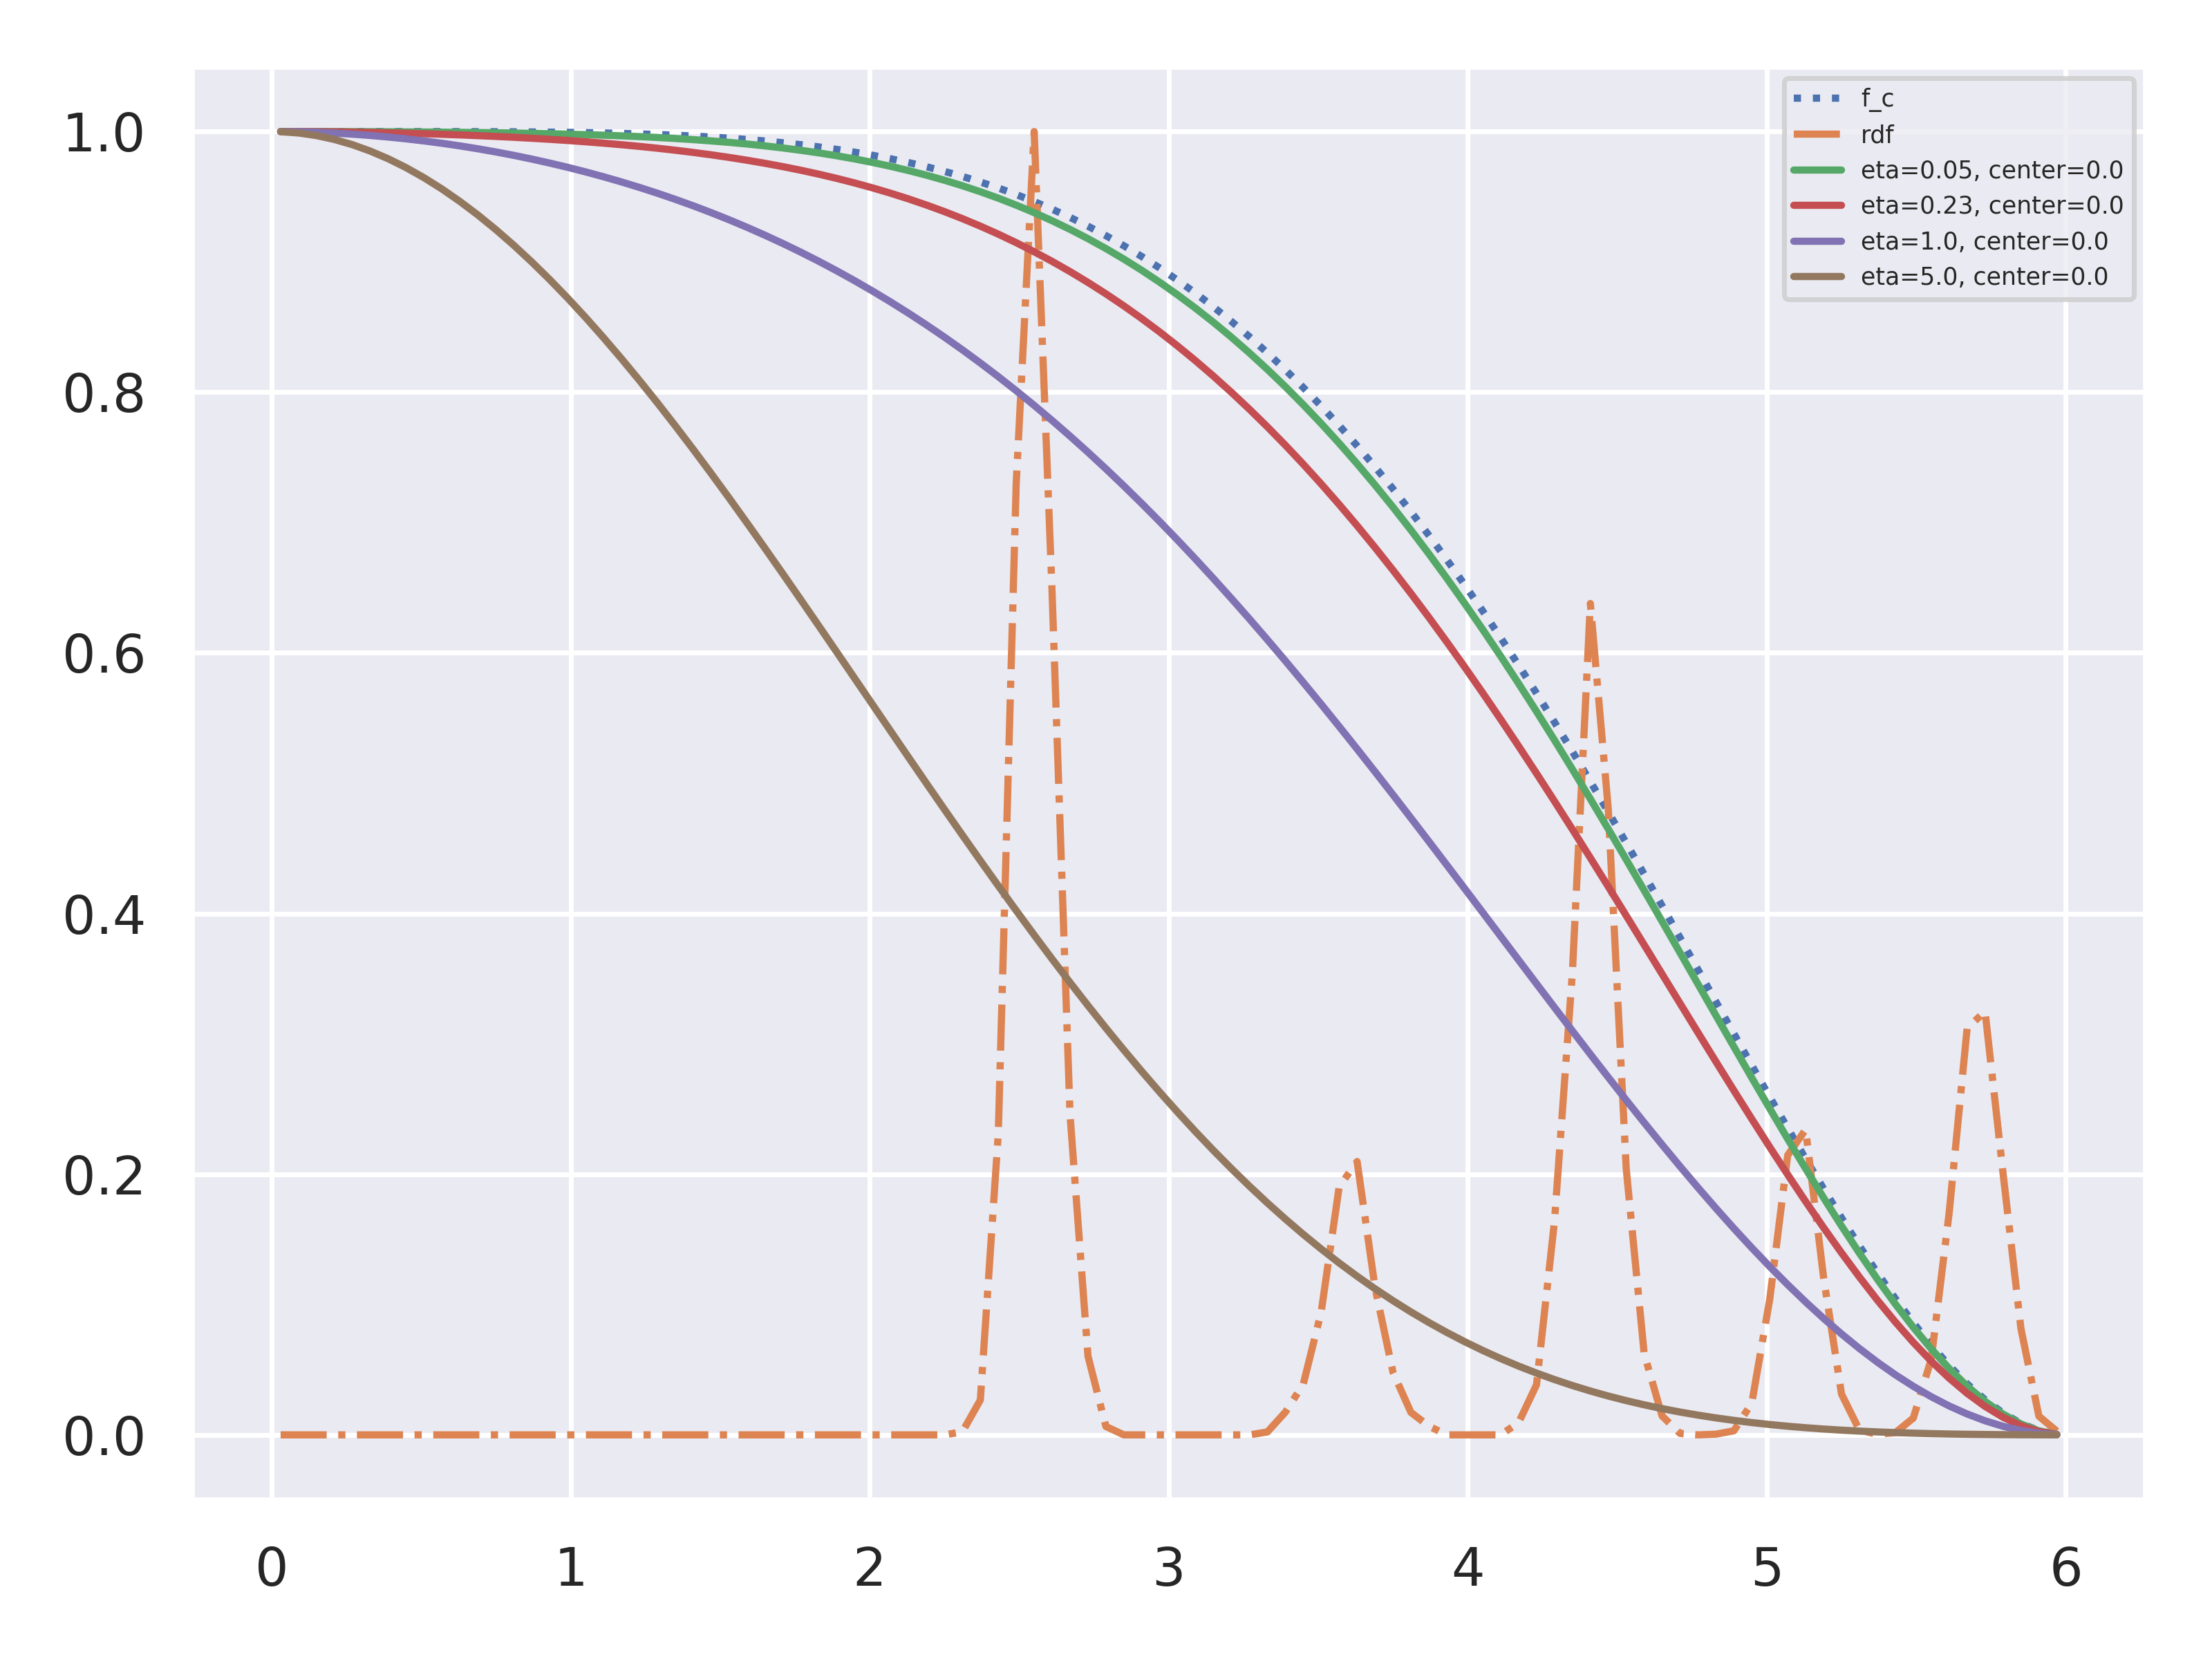
\includegraphics[width=\textwidth]{Default-rad.png}
    \caption{Flower one.}
    \label{fig:f1}
  \end{subfigure}
  \hfill
  \begin{subfigure}[b]{0.55\textwidth}
      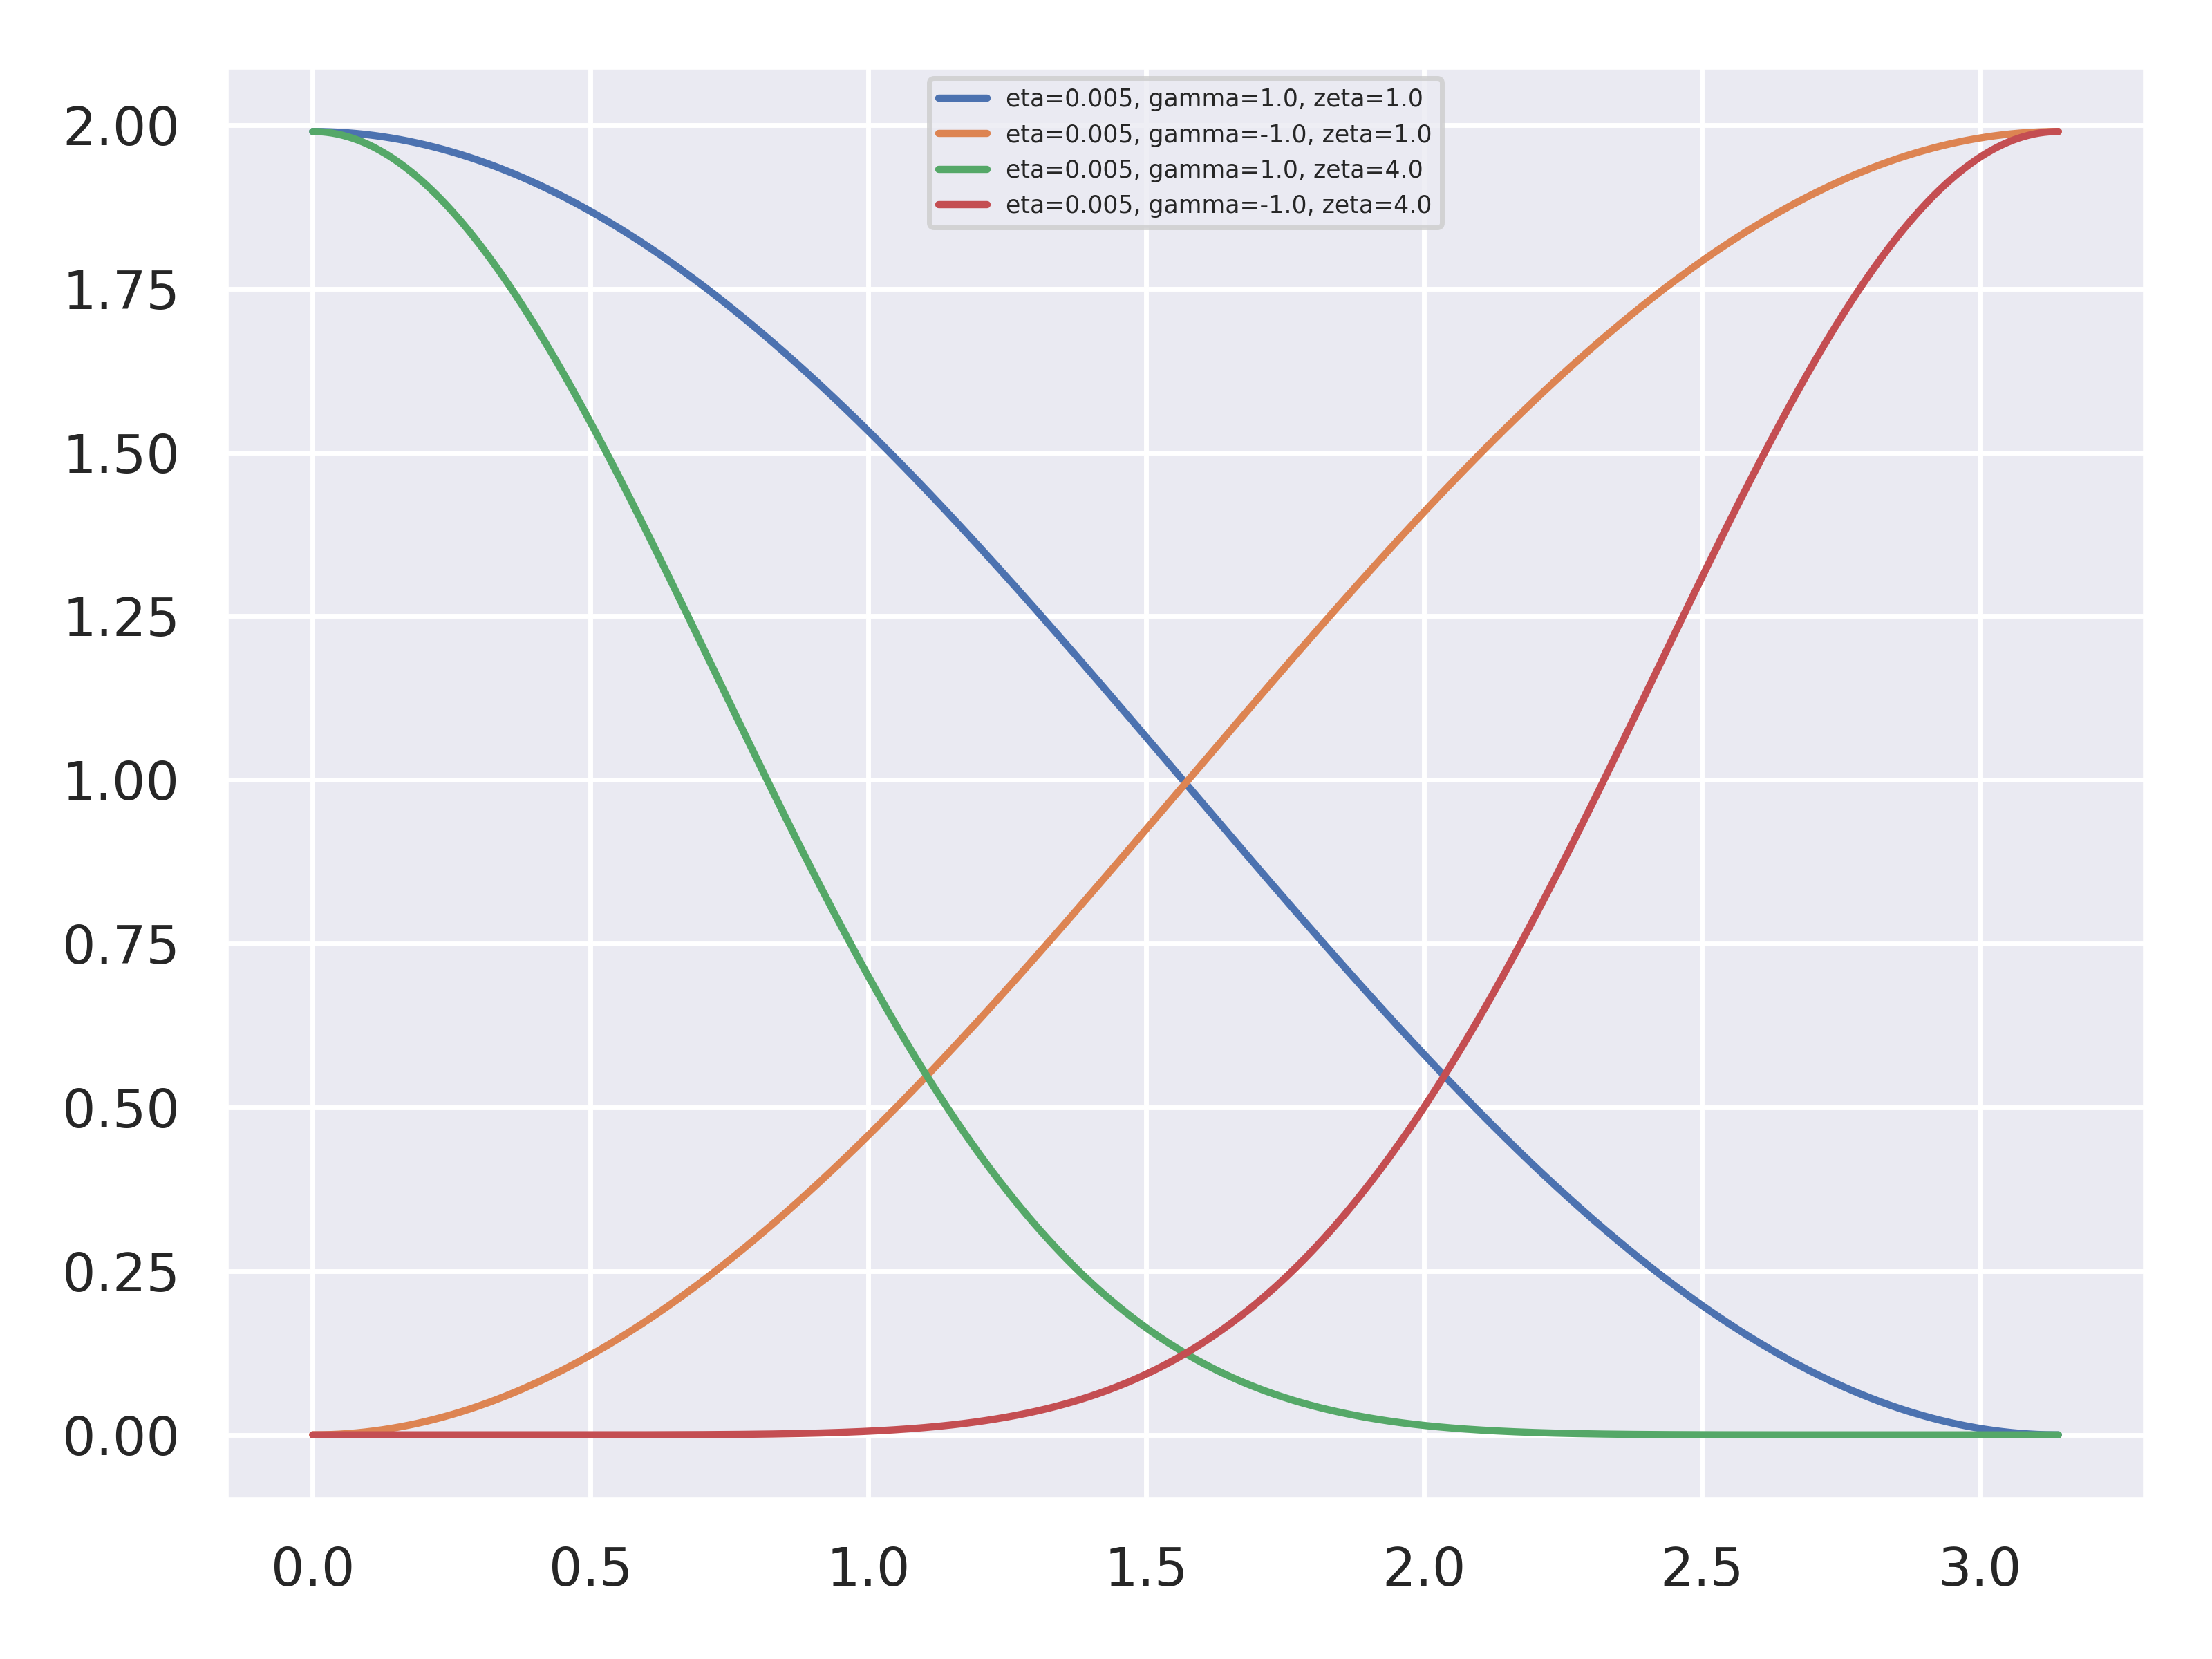
\includegraphics[width=\textwidth]{Default-ang.png}
    \caption{Flower two.}
    \label{fig:f2}
  \end{subfigure}
\end{adjustbox}
\caption{My flowers.}
\end{figure}

\begin{table}
\begin{tabular}{lrr}
\toprule
Symmetry function &  Energy RMSE &  Force RMSE \\
\midrule
          Default &     1.99E-02 &    8.97E+00 \\
      Gs-4-8-1-G4 &     2.26E-03 &    8.65E-02 \\
      Gs-4-8-1-G5 &     2.44E-03 &    1.91E-01 \\
      Gs-5-9-1-G4 &     2.07E-03 &    3.01E-01 \\
      Gs-5-9-1-G5 &     2.59E-03 &    8.02E-02 \\
     Gs-6-10-1-G4 &     1.88E-03 &    1.35E-01 \\
     Gs-6-10-1-G5 &     2.45E-03 &    1.50E-01 \\
     Gs-7-11-1-G4 &     1.78E-03 &    4.13E-02 \\
     Gs-7-11-1-G5 &     2.34E-03 &    1.85E-01 \\
     Gs-8-12-1-G4 &     1.76E-03 &    6.01E-02 \\
     Gs-8-12-1-G5 &     2.51E-03 &    8.92E-02 \\
     Gs-9-13-1-G4 &     2.07E-03 &    6.72E-02 \\
     Gs-9-13-1-G5 &     2.36E-03 &    1.44E-01 \\
    Gs-10-14-1-G4 &     3.80E-03 &    1.27E-01 \\
    Gs-10-14-1-G5 &     2.48E-03 &    4.61E-02 \\
    Gs-10-14-2-G4 &     2.99E-03 &    8.19E-02 \\
    Gs-10-14-2-G5 &     2.31E-03 &    4.98E-02 \\
\bottomrule
\end{tabular}
\caption{Symmetry functions}
\label{table:symmetry}
\end{table}

From these results we observe that not much is gained with respect
to the energy when increasing the number of symmetry functions,
as this space tends be covered reasonably well.
However, we may be able to achieve a lower force RMSE
with adding more symmetry functions, since the forces generally
represent a small perturbation in the position of a single atom,
and this may be better represented by having a larger amount
of functions sensitive to this change. The G4 functions generally
outperform marginally on the force RMSE, and a little poorer
on the energy RMSE.
As for the number of zetas, we only test two values with
$\zeta = 1, 2$, thus doubling the number of angular symmetry functions,
and this seems to make the performance somewhat worse, as we 
might have predicted.

\subsection{Sampling and scaling}
In order for the neural network to learn patterns from data
the data needs to be of high quality, and atomic configurations
should be sufficiently distinguishable while being representative
of the underlying distribution. Neural networks typically perform
poorly or unexpectedly on unseen data, in addition to being data-hungry
requiring fairly large amounts of data in order to train well
over many epochs.
One approach to learning atomic configurations might be to generate
random configurations (not too closely spaced) and calculate energy
and forces from these using a suitable calculator. However, this
phase space of configurations would be enormous using only a few particles,
and we would encounter many highly unlikely configurations.
Since we want to train the neural network to perform molecular dynamics,
the obvious solution is to sample configurations from molecular dynamics
trajectories. However, these configurations are (mostly) in equilibrium, with
relatively small forces, and thus the network might struggle if
it encounters smaller distances between atoms.
In their paper on fitting potential energy surfaces using neural networks,
\parencite[Pukrittayakamee et al.]{pukrittayakamee2009simultaneous}
suggest using a variable time interval dependent on the maximum acceleration:

\begin{equation}
    \tau = 
    \begin{cases}
        \text{trunc}[\alpha / a_{max}]\Delta t & \text{trunc}
        [\alpha / a_{max}] > 0 \\
        \Delta t & \text{trunc}
        [\alpha / a_{max}] = 0
    \end{cases}
\end{equation},

where $\Delta t$ is a minimum time interval and $\alpha$ is a parameter
which must be determined empirically.
The rationale behind this is that we will sample more from
areas where the forces are large, while skipping areas
where the forces are small.
In our experiments using this algorithm (slightly modified)
we find that appropriate choices of $\Delta t$ and $\alpha$
can broaden the distribution of force somewhat, however
it does not add a substantial amount of larger forces, since
these are simply not present in equilibrium.
Other sampling algorithms have been suggested, for example iteratively
pruning a large data set of images where the energy or force 
difference is not very large, and then retraining until
we are satisfied with the result.
One can also check for images where new values of the fingerprints
are encountered and add these to the training set, or checking
images for large overall values of the feature vector. However
these sampling methods have not been tested in this thesis.
Other methods such as metadynamics \footnote{
\url{https://parrinello.ethz.ch/research/metadynamics.html}}
have seen increasing application and there are now numerous implementations
available such as PLUMED \footnote{\url{https://www.plumed.org/}}.
In general, though sampling has not been studied closely in this thesis,
an increase in high quality data is an obvious increase in neural network
performance, both for electronic structure calculations
and for other similar applications.
\par
Neural networks are known as data-hungry, and typically require
a large amount of data to perform well and also scale well
with the number of data points. In order to test this we train a neural
network on progressively larger sets of images generated from molecular dynamics,
and evaluate them on a test set.
The results are shown in table \ref{table:images}.

\begin{table}
\begin{tabular}{lrr}
\toprule
Number of images &  Energy RMSE &  Force RMSE \\
\midrule
             n10 &     8.83E-02 &    7.88E-01 \\
             n20 &     9.40E-02 &    3.79E-01 \\
             n50 &     1.51E-02 &    1.51E-01 \\
            n100 &     6.05E-03 &    4.91E-01 \\
            n200 &     1.96E-03 &    6.95E-02 \\
            n500 &     1.40E-03 &    1.15E-01 \\
           n1000 &     1.41E-03 &    1.60E-01 \\
           n2000 &     1.31E-03 &    1.04E-01 \\
           n5000 &     1.23E-03 &    9.65E-02 \\
\bottomrule
\end{tabular}
    \caption{Number of images}
    \label{table:images}
\end{table}

From these results we see that the energy RMSE scales favorably as
the number of images available increase, and the force RMSE decreases
as well, though not as systematically, due to stochasticity and
the fact that the networks have not been trained on force.
Since these images are sampled directly from molecular dynamics
at constant intervals, this suggests that we can in fact increase
the performance of the neural networks by simply increasing the simulation
length, though obviously more efficient sampling algorithms
should be considered eventually.
